\chapter{Relaxation of integrals of motions in weakly perturbed XXZ model}
\thispagestyle{chapterBeginStyle}

So far we have focused on investigating properties of an \textit{integrable} XXZ
spin-\(1/2\) chain.
\textcolor{blue}{Write, this part after the introduction to avoid repetition.}
It is important to note, that the methodology in this chapter follows the work
of~\textcite{Mierzejewski2015Approx}, however the results about relaxation of noncommuting integrals
of motion are original and at the moment of writing this thesis not found elsewhere
in literature. 
\textcolor{blue}{derivation of \(I(\omega)\)? autocorrelation only for \(t>0\)?}
\section{Adding perturbation to the Hamiltonian}
We are now going to weakly break integrability by adding a suitable perturbation.
New Hamiltonian has the following form:
\begin{equation}
    H_{XXZ} = \frac{1}{2}\sum_{j = 1}^{L}\left( S^{+}_{j} S^{-}_{j+1} + 
    S^{-}_{j}S^{+}_{j+1} \right) + \Delta\sum_{j = 1}^{L} S^{z}_{j}S^{z}_{j+1}
    + \alpha H'
    \label{eq:HXXZ perturbed}
\end{equation}
where \(H'\) is the perturbation that breaks integrability for nonzero \(\alpha \):
\begin{equation}
    H'=\sum_{j = 1}^{L} S^{z}_{j}S^{z}_{j+2}
    \label{eq:perturbation}
\end{equation}
In such system, only two conserved quantities remain --- the Hamiltonian \(H_{XXZ}\) itself 
and the total magnetization \(\Sz_{tot}\). All other integrals of motions cease to be conserved
and decay with a finite relaxation time \(\tau\). We are interested in investigating this
decay and the timescales involved. However at first we should establish a range of
values of parameter \(\alpha\) so its small enough that \(H'\) remains a perturbation
but large enough to be relevant for finite system sizes accessible numerically. 
To this end we take the previously discussed (Q)LIOMs  \(J^E, \hat{O}_1,\hat{O}_2\)
and investigate their behavior under finite-time averaging (as defined in~\eqref{def:simple time avg})
generated by perturbed Hamiltonian. More precisely, we calculate the finite-time autocorrelation
function (finite-time stiffness) \(\lambda^{\tau}_A = \hs{\bar{A}^{\tau}}{\bar{A}^{\tau}}\) as
a function of inverse system size.
In order to relate this to the discussion of spectral functions in Section~\ref{sec:spectral function},
we will from now on use the cutoff frequency \(\omega = \frac{1}{\tau}\), instead of the time of
averaging \(\tau\). 

\begin{figure}[htbp]
  \centering
  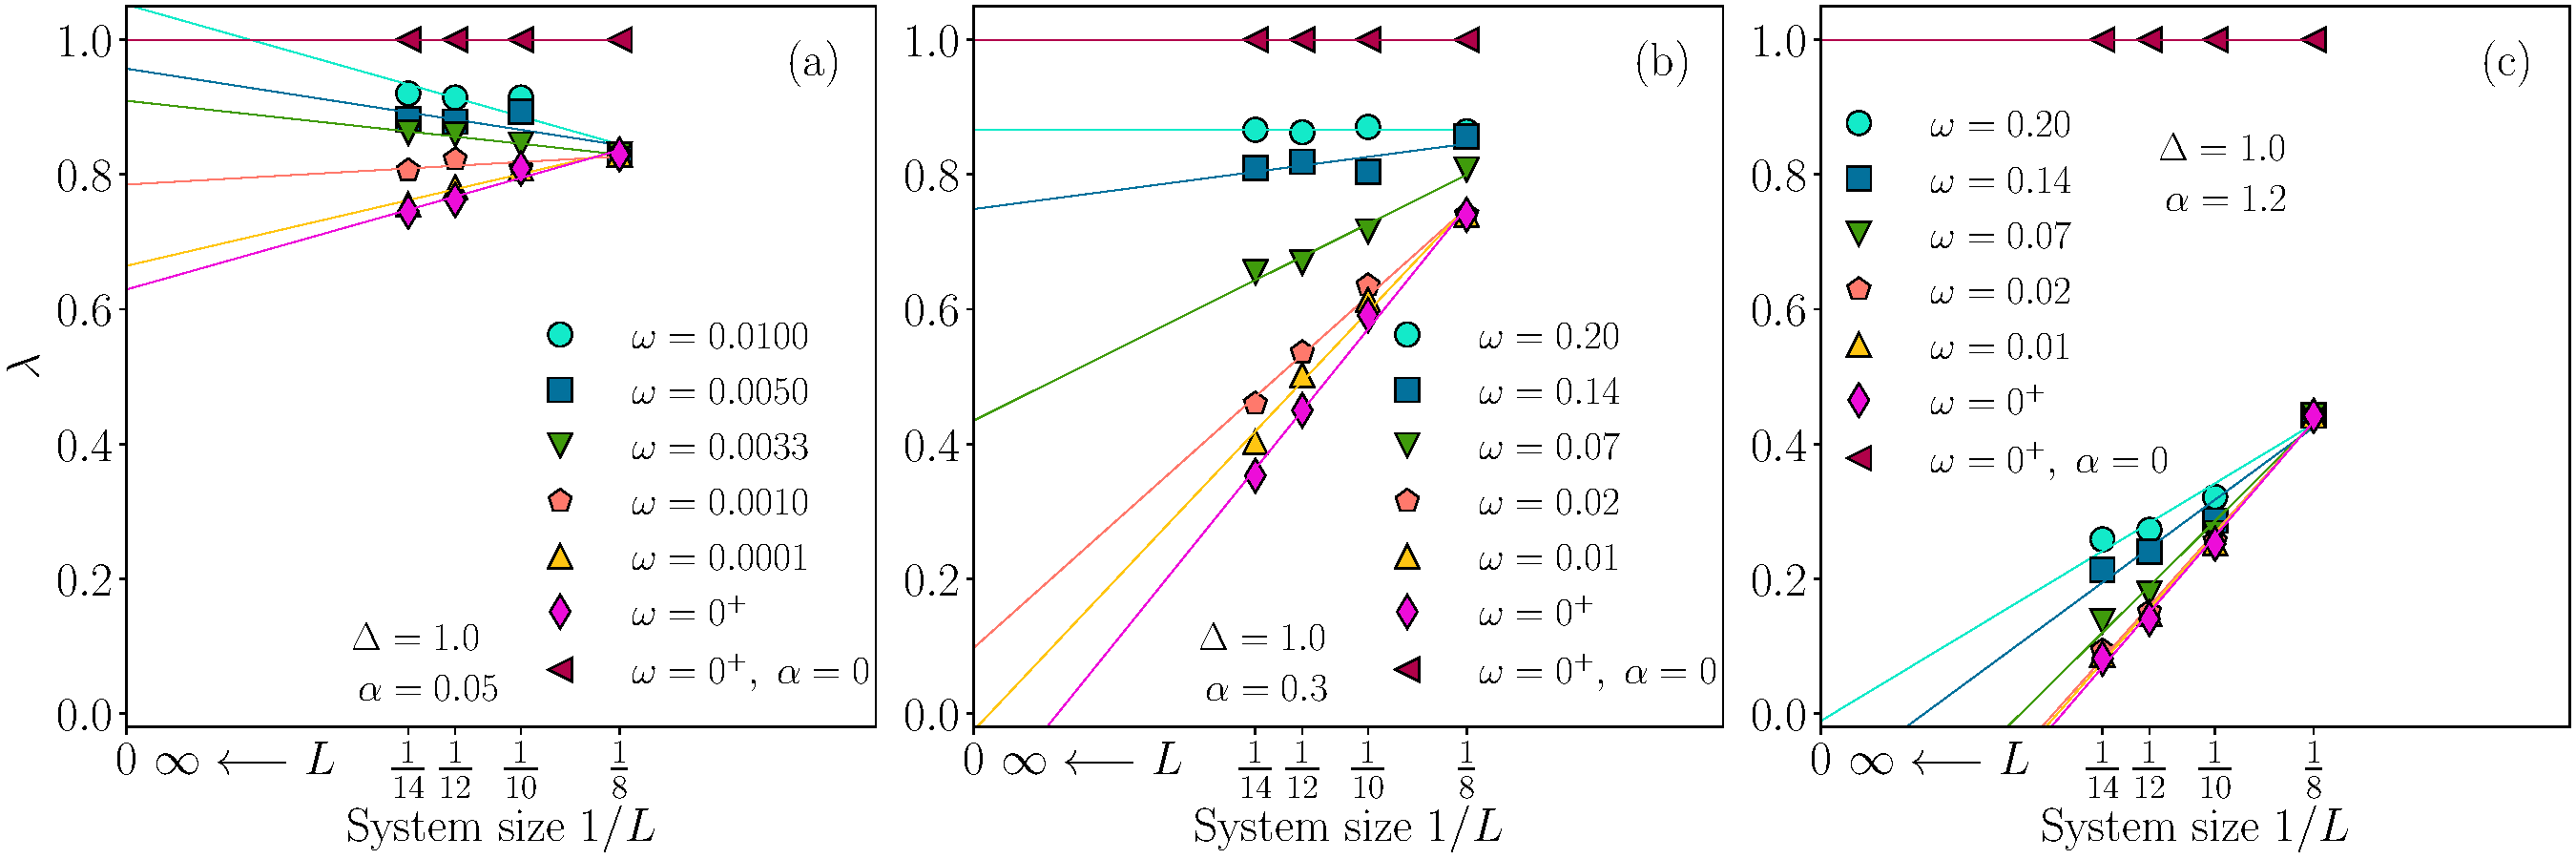
\includegraphics[width=\textwidth]{Figures/current_decay.pdf}
  \caption{Finite time stiffness of \(J^E\) as a function of time for the perturbed Hamiltonian.
  Perturbation strength increase from left to right \(\alpha=0.05,0.3,1.2\).
  (a) Perturbation is too weak and even for very small \(\omega\) the stiffness does
  not vanish. (b) Optimal perturbation, stiffness vanish for suitably small cutoff frequency.\\
  (c) Perturbation too strong, stiffness vanish almost immediately.}
  \label{fig:current decay}
\end{figure}





\newpage

\section{Relaxation of known (Q)LIOMs}
After establishing the range of perturbation strengths relevant to our problem, we can now
investigate how our (Q)LIOMs decay with time. We will apply the formalism of spectral functions
described in Sections~\ref{sec:spectral function}.
Since we are interested in the low-\(\omega\) (long times) part of integrated spectral function
\(I(\omega)\), it is convenient to normalize it. Therefore, let us define the
following~\autocite{Mierzejewski2015Approx}:
\begin{equation}
  R_{\hat{A}}(\omega,\alpha) = \frac{I(\omega,\alpha)}{\lim_{\omega \to 0^{+}} I(\omega,\alpha=0)} = 
  \frac{\sum_{n,m}\theta\left(\omega -\abs{E_n-E_m}\right) \abs*{\matrixel{m}{\hat{A}}{n}}^2}
  {\sum_{\substack{n,m \\ E_n=E_m}} \abs*{\matrixel{m}{\hat{A}}{n}}^2}
  \label{eq:integrated spectral function}
\end{equation}
This normalization of \(I(\omega)\) assures that 
\(\lim_{\omega\to 0^{+}} R_{\hat{A}}(\omega,\alpha) = 0\) and 
\(\lim_{\omega\to \infty} R_{\hat{A}}(\omega,\alpha) = 1\). Let us now study this quantity
for operators in question.


\section{Relaxation of energy current}
\textcolor{blue}{\(\Delta=0.5\)?}
We begin with the case energy current \(J^E\) for \(\Delta = 1.0\), as derived in Section~\ref{sec:energy current}.
In the integrable parent model it is a conserved quantity, so we have the following:
\begin{equation*}
  \hs{J^E(t)}{J^E} = const \implies S(\omega) \propto \delta(\omega)
  \implies R_{J^E}(\omega,\alpha=0) = 1
\end{equation*}
After moving away from integrable regime, the autocorrelation function starts to decay,
so the \(\delta\)-peak broadens and \(R_{J^E}(\omega,\alpha=0)\) is no longer equal to one,
but approaches zero as time increases. We will look simultaneously at two different situations,
results for \(L=14\) and results extrapolated to thermodynamic limit from \(L=11,12,13,14\). 
Figure~\ref{fig:current decay no scaling} shows \(R(\alpha,\omega)\) as a
function of \(\omega\) for different \(\alpha\). We immediately see the expected outcome, as the stronger
the perturbation the faster the current decays.
\begin{figure}[htbp]
  \centering
  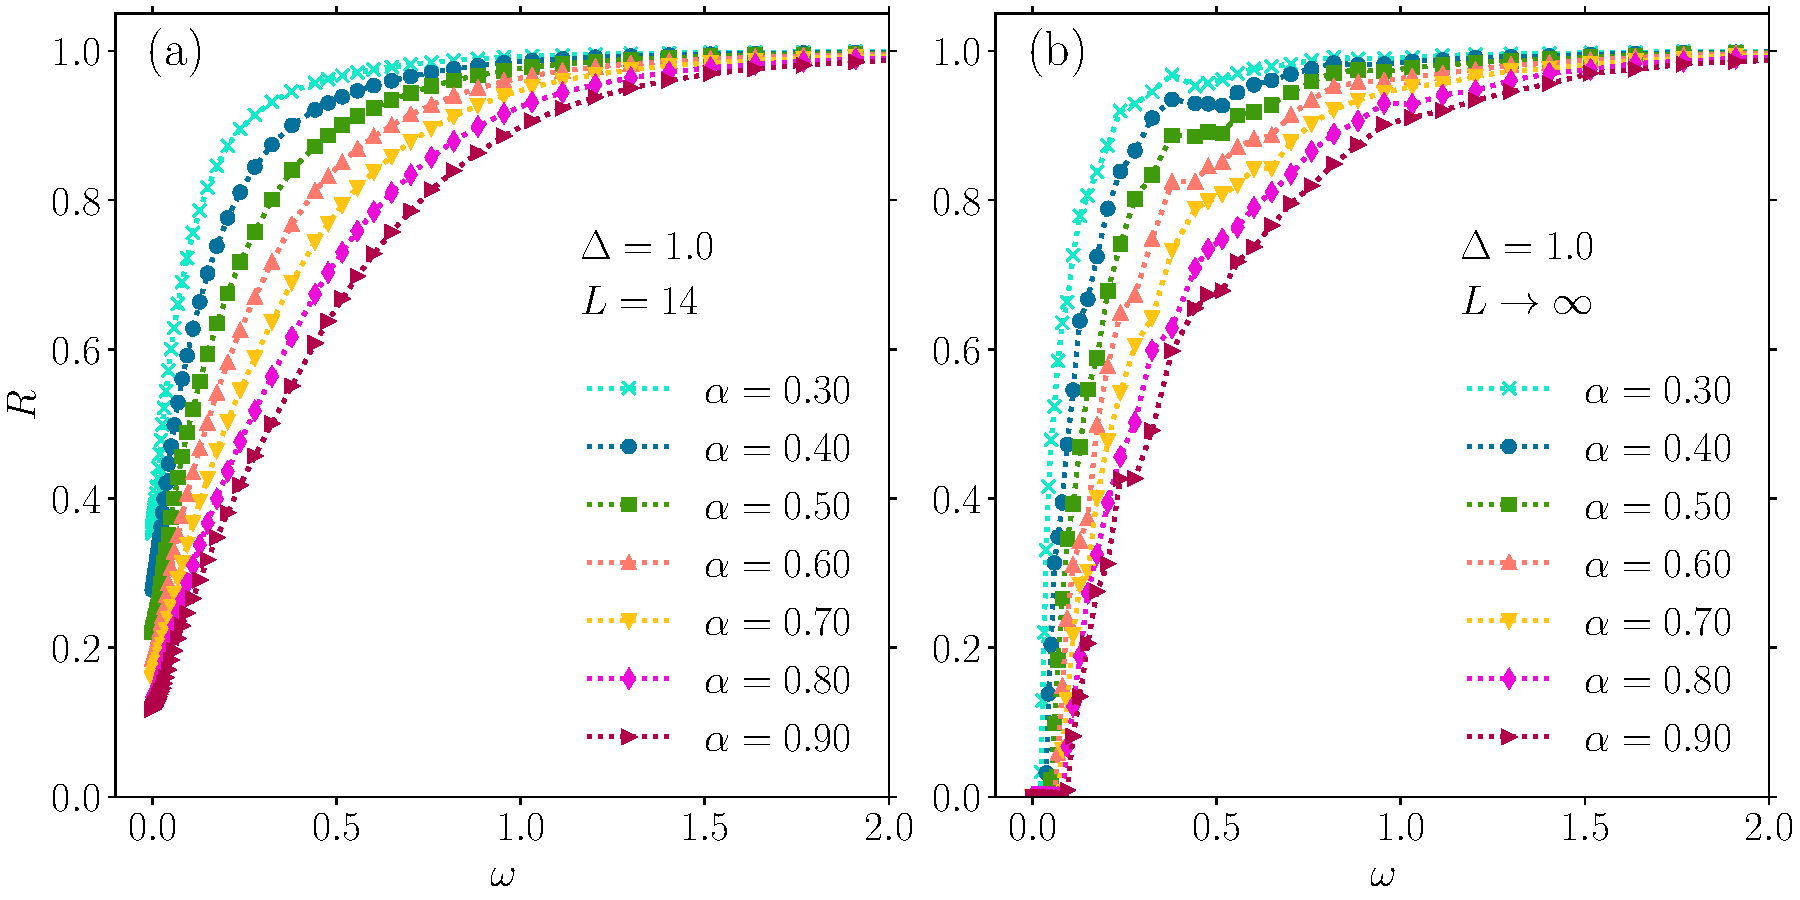
\includegraphics[width=\textwidth]{Figures/current_no_scaling.pdf}
  \caption{Normalized integrated spectral function as a function of cutoff frequency.
  (a) Results for \(L=14\). Low frequency limit does not approach 0
  because of finite size effects. (b) Results extrapolated to thermodynamic limit from \(L=11,12,13,14\).
  Note the expected observation, namely stronger perturbation leads to faster decay.}
  \label{fig:current decay no scaling}
\end{figure}
However, an interesting thing happens when plot the same data, but as a function of rescaled
frequency \(\omega/\alpha^2\). Numerical results visible on Figure~\ref{fig:current decay scaling}
show a convincing collapse of curves for different values of perturbation strength. This may suggest
an universal dependence of \(R(\omega,\alpha)\) on \(\omega\) and \(\alpha\):
\begin{equation}
  R(\omega,\alpha)\simeq \tilde{R}(\omega/\alpha^2)
\end{equation}
Moreover, this relation can be reasonably well approximation by a one parameter fit
(black dashed line on Figure~\ref{fig:current decay scaling}):
\begin{equation}
  \tilde{R}(\omega/\alpha^2) \simeq \frac{2}{\pi} \arctan\left(\frac{\omega}{\gamma \alpha^2}\right)
\label{eq:R arctan}
\end{equation}
where \(\gamma \) is the fitting parameter. It implies that the relaxation of energy current
is exponential in nature. To see this, let us calculate \(I(\omega)\) for such decay
\(\hs{J^E(t)}{J^E} \propto e^{-\abs{t}/\tau_1}\). Double-sided exponential has well defined Fourier
transform, so we can drop the \(\epsilon \to 0^{+}\) limit from the integral.
\begin{align}
  S(\omega) &\propto \frac{1}{2\pi} \int_{-\infty}^{\infty} \mathrm{d} t\; e^{-\abs{t}/\tau_1} e^{i \omega t} = 
  \frac{1}{2\pi} \left[\int_{-\infty}^{0} \mathrm{d} t\; e^{(1/\tau_1 + i\omega)t }
  + \int_{0}^{\infty} \mathrm{d} t\; e^{(-1/\tau_1 + i\omega)t }  \right] \nonumber \\
  &= \frac{1}{2\pi} \left[\frac{\tau_1}{1+i\omega \tau_1} + \frac{\tau_1}{1-i\omega\tau_1}\right] = 
  \frac{1}{\pi} \frac{\tau_1}{1+\omega^2\tau_1^2}
\end{align}
Integrating \(S(\omega)\) over a frequency window we obtain:
\begin{equation*}
  I(\omega) \propto \frac{1}{\pi}\int_{-\omega}^{\omega}\mathrm{d}\omega^{\prime}\; 
  \frac{\tau_1}{1+\omega^2\tau_1^2} = \frac{2}{\pi} \arctan(\tau_1 \omega)
\end{equation*}
which after normalization yields the desired results~\eqref{eq:R arctan}. Furthermore, we learn that the 
characteristic relaxation time \(\frac{1}{\tau_1} \propto \alpha^2\) and the proportionality
coefficient is universal and does not depend on \(\alpha\).
\begin{figure}[htbp]
  \centering
  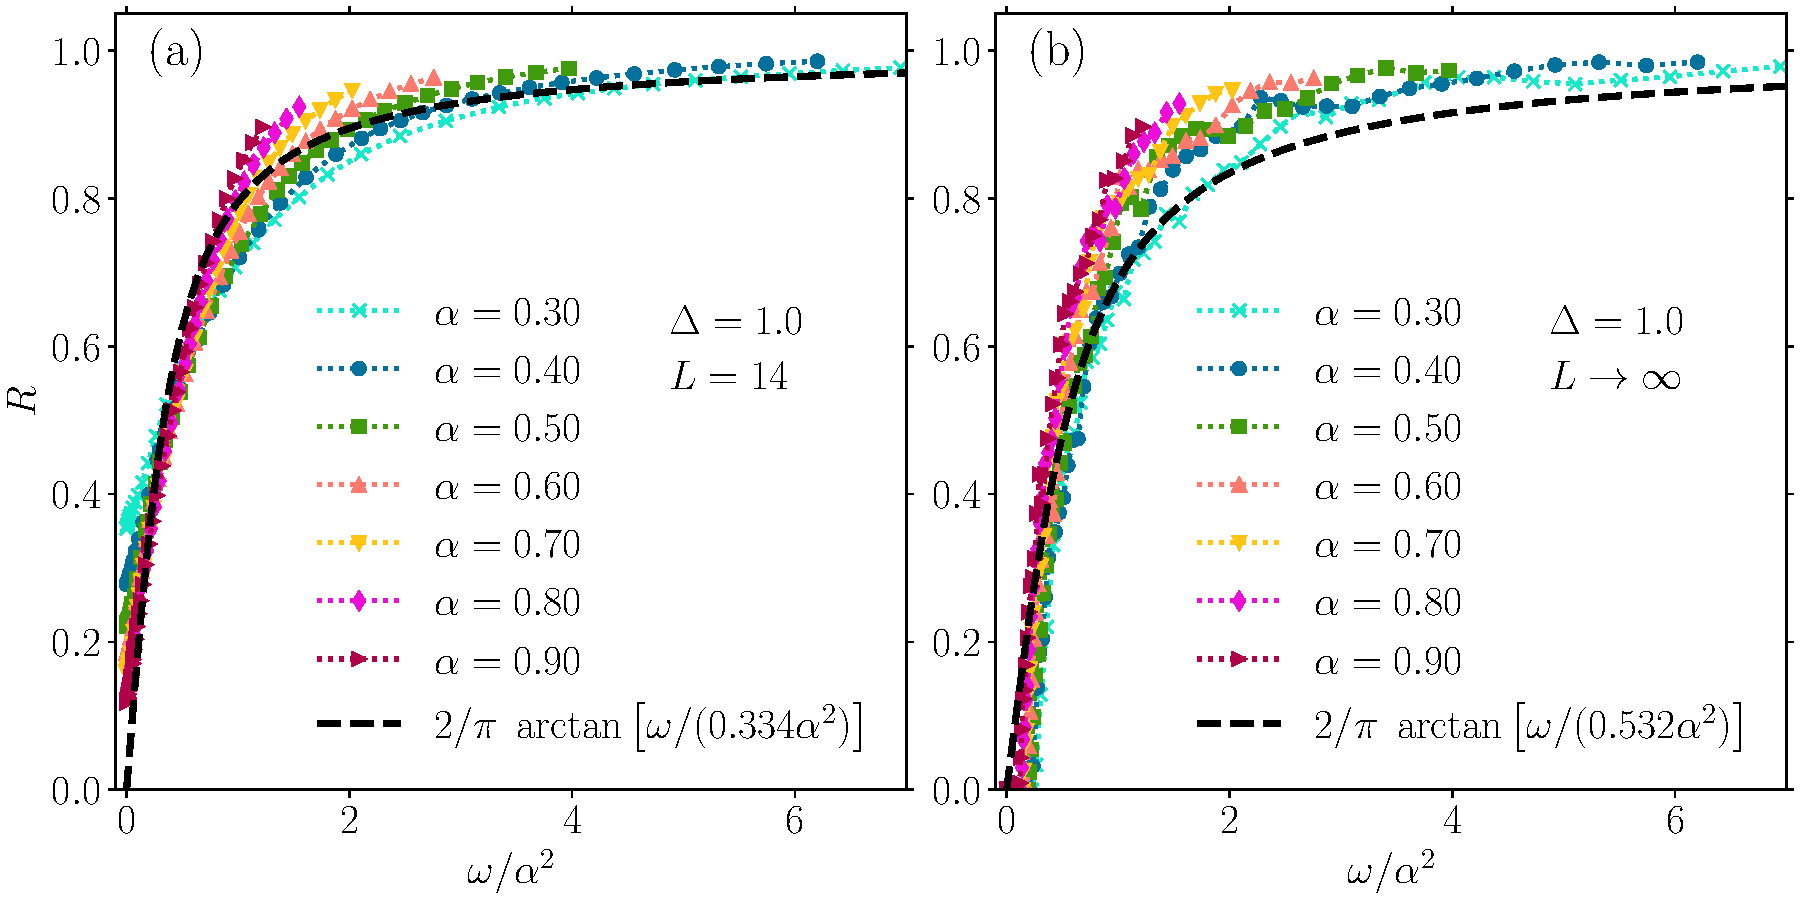
\includegraphics[width=\textwidth]{Figures/current_scaling.pdf}
  \caption{Normalized integrated spectral function as a function of rescaled cutoff frequency.
  (a) Results for \(L=14\). (b) Results extrapolated to thermodynamic limit from \(L=11,12,13,14\).
  Dashed black line corresponds to fit~\eqref{eq:R arctan}.}
  \label{fig:current decay scaling}
\end{figure}
The quadratic scaling shown on Figure~\ref{fig:current decay scaling} is actually not the
best possible for this set of numerical data. Choosing the rescaling coefficient to be
\(\frac{3}{2}\) allows for almost perfect collapse of all the curves 
(see Figure~\ref{fig:current decay perfect scaling}). However, it is expected to be a consequence
of working with rather small system sizes, because in was shown 
in~\textcite{Mierzejewski2015Approx} using memory function formalism, that quadratic scaling
is indeed the appropriate one.
\begin{figure}[htbp]
  \centering
  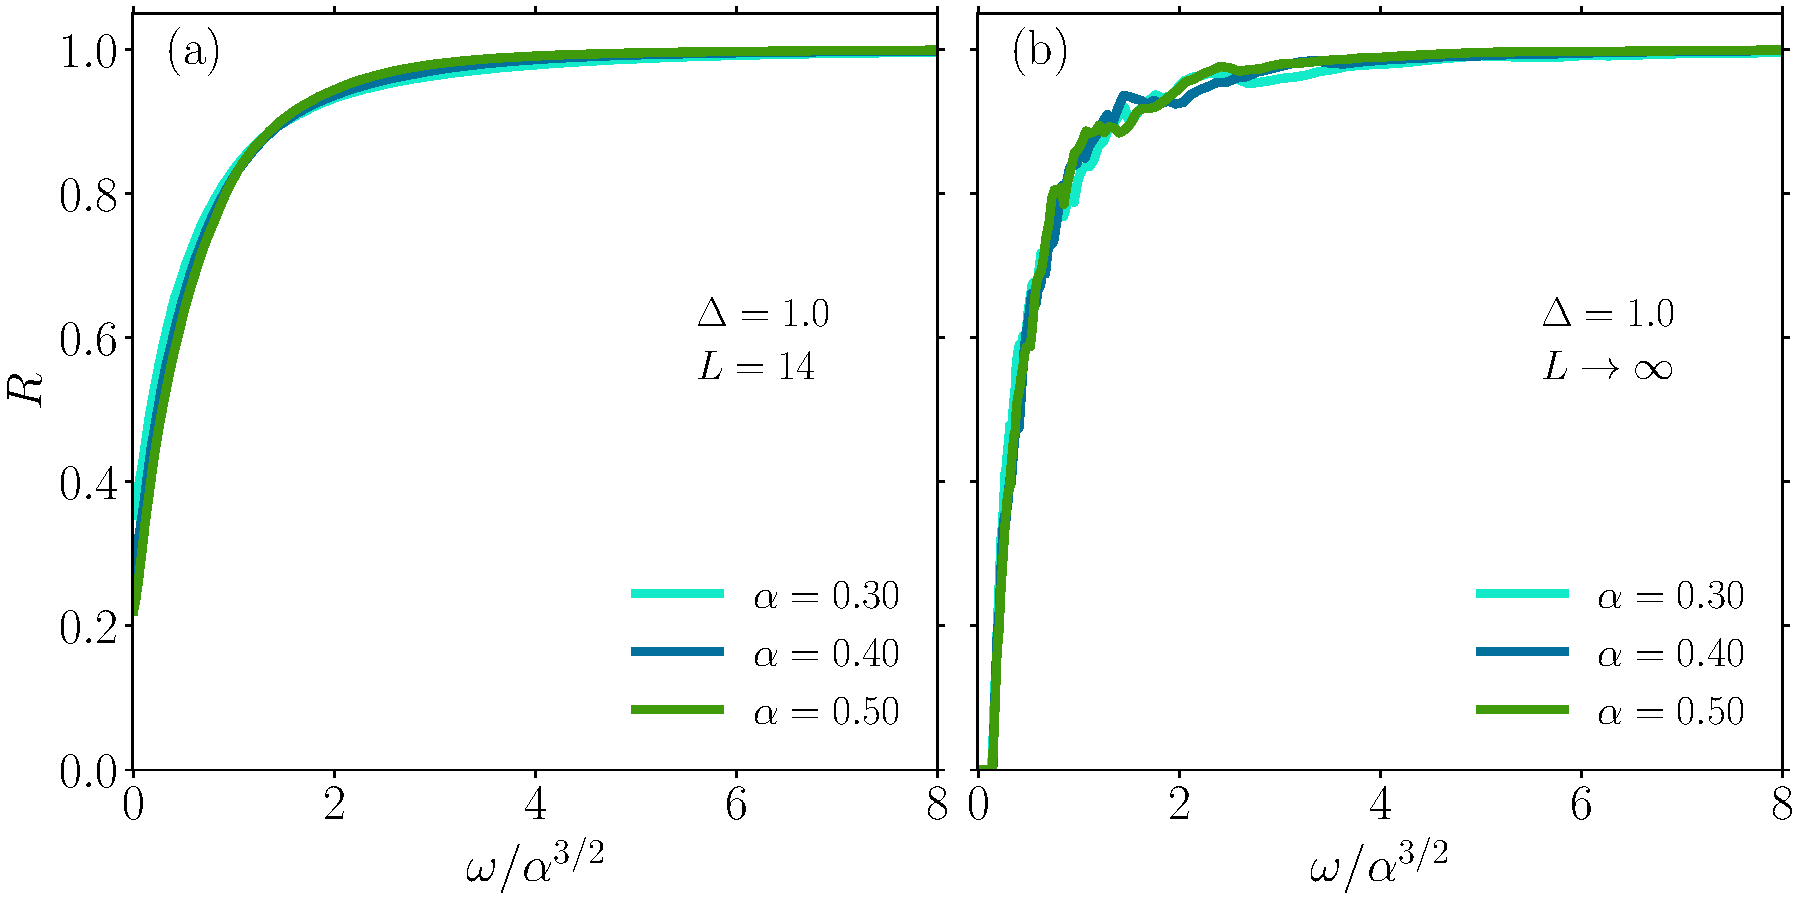
\includegraphics[width=\textwidth]{Figures/current_perfect_scaling.pdf}
  \caption{Normalized integrated spectral function as a function of 
  rescaled cutoff frequency. The rescaling coefficient is chosen so as to obtain the 
  best possible collapse of curves. (a) Results for \(L=14\). (b) Results extrapolated
   to thermodynamic limit from \(L=11,12,13,14\).}\label{fig:current decay perfect scaling}
\end{figure}



\section{Relaxation of noncommuting (Q)LIOMs}
Let us now proceed with the same analysis, but for the \(\hat{O}_1\) and \(\hat{O_2}\)
operators.

\textcolor{blue}{What to show here?
\begin{itemize}
  \item no scaling, quadratic scaling, linear scaling
  \item fitting error function, derivation of \(I(\omega)\)
  \item SU(2) breaking for \(\Delta=1.0\)
  \item for \(\Delta = 0.5\) too? why?
  \item loglog plots?
  \item comparison between SU(2) breaking and integrability breaking
\end{itemize}
}